These are the results of the various algorithms we have implemented.
Starting off with the KNN and Nearest Centroid algorithms, we get:
\begin{figure}[H]
    \centering
    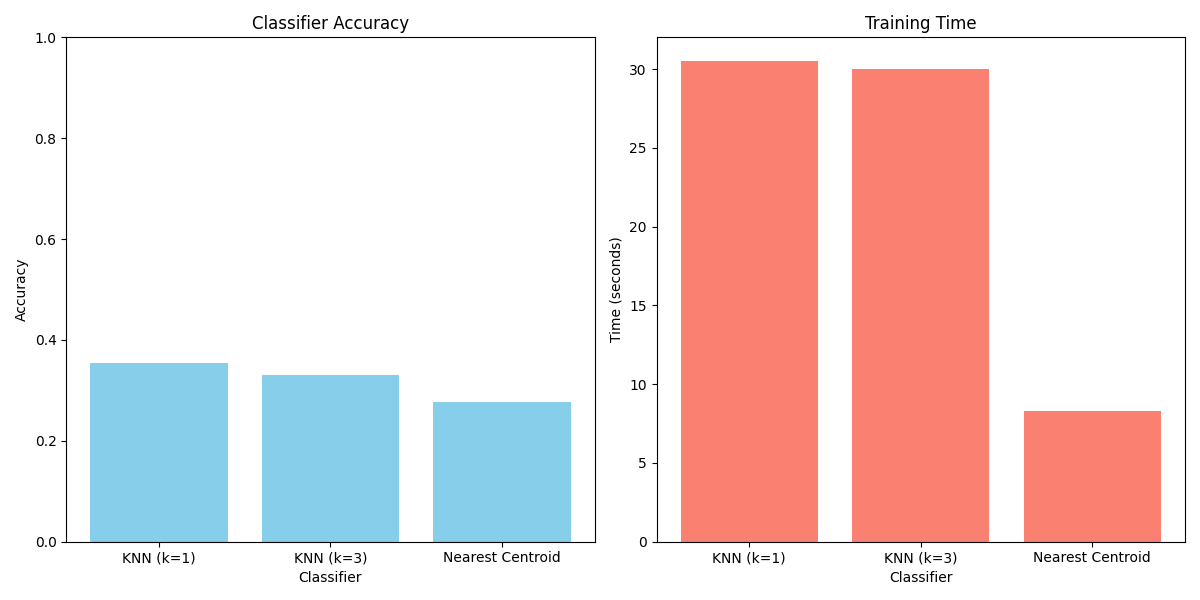
\includegraphics[width=0.5\textwidth]{media/knn_centroid.png}
    \caption{KNN Centroid Graph}
\end{figure}

Moving on to the MLP and CVM algorithms, it is important to note that
we are using:
\begin{itemize}
    \item A CPU as the training device
    \item Activation function: ReLU
    \item Loss function: Hinge loss
    \item Optimizer: Adam 
    \item Learning rate: 0.001
    \item Learning rate scheduler: ReduceLROnPlateau 
    \item Epochs: 30
    \item Training batch size: 128
    \item Testing batch size: 256
\end{itemize}

The graphs for both algorithms are as follows:
\begin{figure}[H]
    \centering
    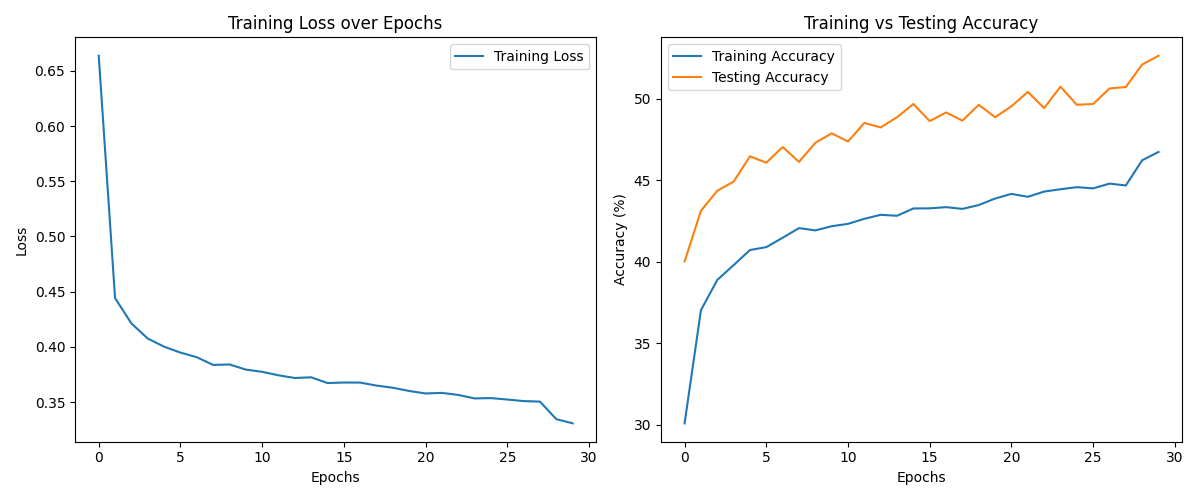
\includegraphics[width=0.5\textwidth]{media/mlp.png}
    \caption{MLP Graph}
\end{figure}

\begin{figure}[H]
    \centering
    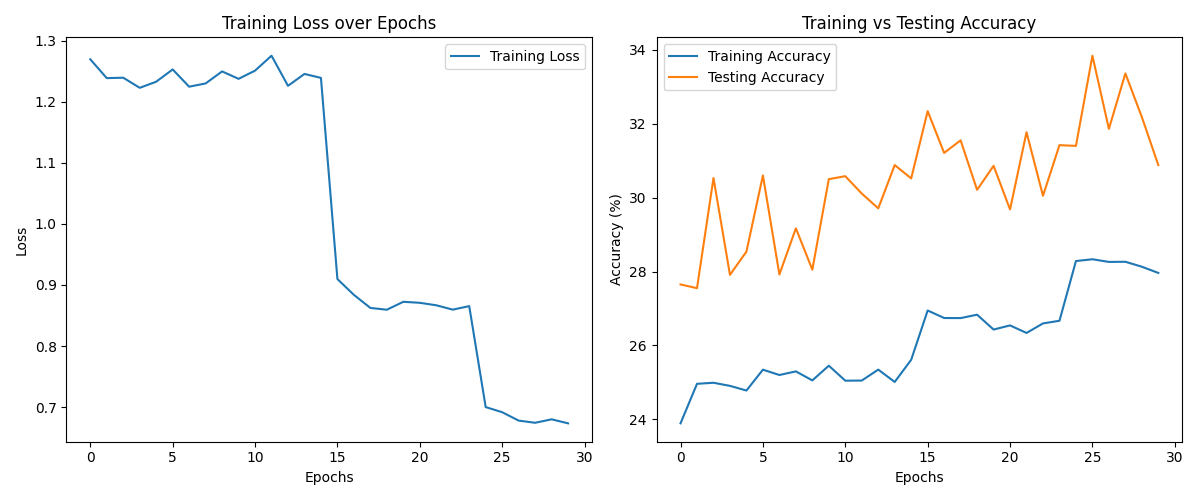
\includegraphics[width=0.5\textwidth]{media/svm.png}
    \caption{SVM Graph}
\end{figure}
Randomization filter like cropping and flipping improves the model's performance
but in return the training accuracy drops below the testing accuracy.\\

\smallskip

Lastly, the collective results showing the accuracies and times of
each algorithm, side by side, are as follows:
\begin{table}[H]
    \centering
    \begin{tabular}{|c|c|c|}
        \hline
        Algorithm & Accuracy & Time (seconds) \\
        \hline
        1-NN & 35.39 & 30.50 \\
        3-NN & 33.03 & 30.01 \\
        Nearest Centroid & 27.74 & 8.27 \\
        MLP & 52.63 & 1184.4 \\
        SVM & 33.84 & 321 \\
        \hline
    \end{tabular}
    \vspace{0.5cm}
    \caption{Comparison of Algorithms}
\end{table}

As an attempt to see if the algorithms have potential to rise in accuracy,
I increased the number of epochs:
\begin{figure}[H]
    \centering
    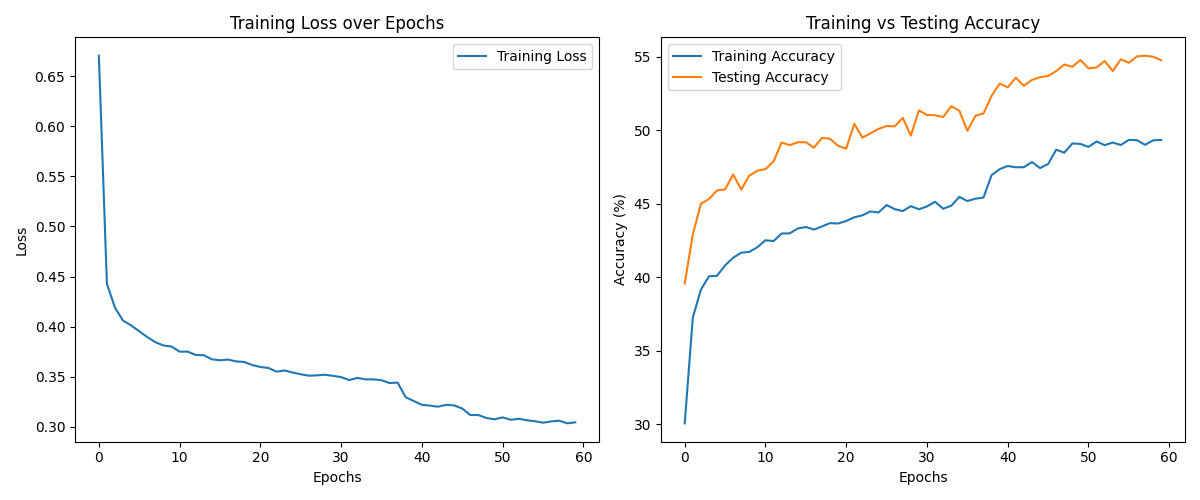
\includegraphics[width=0.5\textwidth]{media/mlp_max.png}
    \caption{MLP Graph - Extended Edition}
\end{figure}
Training completed in 43.65 minutes \\
Best accuracy: 55.08\% \\

\begin{figure}[H]
    \centering
    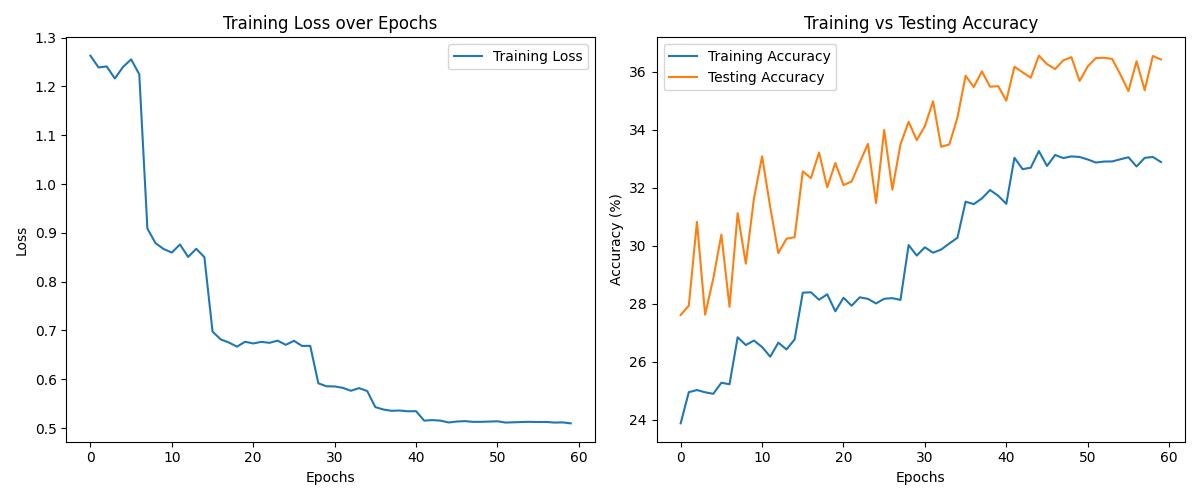
\includegraphics[width=0.5\textwidth]{media/svm_max.png}
    \caption{SVM Graph - Extended Edition}
\end{figure}
Training completed in 10.69 minutes \\
Best accuracy: 36.55\% \\

\smallskip

In the end the improvement was not significant.
